\documentclass[12pt]{article}
\usepackage{graphicx}
\usepackage{subcaption}
\usepackage{amsmath}
\usepackage{amssymb}
\usepackage{amsfonts}

\title{BIOS 611 Final Report - Modeling Cell Migration on Substrates with Differing Stiffness}
\author{Elizabeth Davis}
\date{\today}

\begin{document}
\maketitle

\section{Introduction}

Cell migration is important in many different biological processes, such as morphogenesis, immune response, wound healing, and tumor 
metastasis [1] [2] [3] [4]. 
Cell migration is characterized by an elongation with a leading edge of the cell membrane that contains protrusions. These protrusions
adhere to the substrate the cell is situated on, probe the physical properties of the substrate, and generate forces that ultimately cause 
the rear of the cell to retract, thus leading to overall cell motion [2]. Cell migration has typically been modeled as a persistent 
random walk (PRW), a variation on the random walk but instead of equal probability of moving in any direction at each time step the cell is now more likely to move in the direction of the previous time step.
However, this assumption of the PRW model fails to explain many aspects of the data, such as the non-Gaussian distribution of velocities and the non-singular exponential decay
of the velocity autocorrelation function [4]. Characterizing cell shape and cell motion on substrates of differing stiffnesses and incorporating the two may aid 
in providing insight as to the mechanism cells employ to sense their environment and migrate.

In this analysis, I compare the behavior of cells migrating on two different stiffnesses of substrate: glass and gel. I look at various motion features, such as speed and persistence, and shape features
to try to discern if there is any difference between the behaviors on glass and gel substrates. Lastly,
I develop a model to explain the observed behavior and compare it to the traditional PRW model that is typically used to describe cell migration. I also compare different methods of 
fitting the model.

\section{Cell Migration Data}

This data set comes from DIC 
microscopy images of mesenchymal cells migrating over a period of 20 to 30 hours with 10-
minute intervals between each frame. The cells in this dataset are migrating on two different 
substrate types: gel and glass.  From these movies, the cells are segmented from the 
background and binary masks of the cells are generated. Next, using the centers of the cell 
masks, cell tracks are reconstructed using a closest-neighbor algorithm. Additionally, cell shape 
information is extracted from the masks, such as measures of polarity, area, roundness, etc. 
From the cell tracks, different metrics of cell motion can be extracted, such as velocity, 
measures of persistence (tendency of the cell to move in one direction before switching 
directions) and mean squared displacement. In summary, the raw data used in this analysis is 
pickle files, from which dataframes are extracted that contain $x$ and $y$ coordinates for each track as well as shape features. 
From the coordinates, motion features are calculated as a part of this analysis pipeline and stored as a dataframe. A note here is that I specify
that tracks must contain at least 30 time points. This constraint is used to filter the data so all tracks analyzed have 30 or more time points.

\section{Comparing Motion Features on Glass and Gel}

First, we will look at the comparison of $x$ and $y$ step sizes ($dx$ and $dy$) on glass and gel with a box plot. We calculate
the one-way ANOVA test and find that there is no statistical difference between step sizes on glass and gel (with a threshold of $p < 0.05$ considered
statistically significant) (Fig. 1).

\begin{figure}[h!]
  \centering
  \begin{subfigure}[b]{0.4\linewidth}
    \includegraphics[width=\linewidth]{figures/histogram_boxplot/dx_boxplot.png}
    \caption{Step size ($dx$) on glass vs gel}
  \end{subfigure}
  \begin{subfigure}[b]{0.4\linewidth}
    \includegraphics[width=\linewidth]{figures/histogram_boxplot/dy_boxplot.png}
    \caption{Step size ($dy$) on glass vs gel}
  \end{subfigure}
  \caption{$dx$ and $dy$ do not appear to be statistically different on glass vs. gel.}
\end{figure}

Next, we look at the motion metrics of $D/T$ and speed. $D/T$ is a measure of persistence and is calculated from the net displacement 
divided by the total path length for each track. Speed is simply the total path length divided by the time taken to travel that distance. From the
box plots, we can see that both $D/T$ and speed are statistically different on glass vs gel (Fig. 2). 

\begin{figure}[h!]
  \centering
  \begin{subfigure}[b]{0.4\linewidth}
    \includegraphics[width=\linewidth]{figures/histogram_boxplot/DoverT_boxplot.png}
    \caption{$D/T$ (measure of persistence) on glass vs gel}
  \end{subfigure}
  \begin{subfigure}[b]{0.4\linewidth}
    \includegraphics[width=\linewidth]{figures/histogram_boxplot/speed_boxplot.png}
    \caption{Speed ($\mu m/ \text{min}$) on glass vs gel}
  \end{subfigure}
  \caption{Comparison of motion metrics.}
\end{figure}

\section{Autocorrelation Analysis}

The autocorrelation function is a statistical tool used to compare a time series to a time lagged version of itself. This is done by 
calculating the covariance of time series data (such as velocity) at some time point ($t$) and a later time point ($t + \tau$) divided 
by the variance at time point $t$. Basically, this tells us how correlated something is in time. 

I performed an autocorrelation analysis of velocity (Fig. 4) and polarity (Fig. 3), averaging the autocorrelation over the first 26 time lags. Velocity is a motion metric and polarity is a shape feature. Looking at the
autocorrelation plots, we can see that there is a difference in the decay of the autocorrelation function when comparing glass and gel for both features.
Both the velocity and polarity vector autocorrelation plots have a slower decay time on glass than gel. Additionally, the decay of the autocorrelation plots
do not fit a single exponential function, but rather is indicative of some kind of combination of processes with different time scales. This would possibly explain the 
prolonged decay. (Note: The autocorrelation should decay to zero, but it doesn't here. I hypothesize that this is because I am averaging the autocorrelation
over the first 26 time lags and the short tracks would have decayed to zero already while the long tracks have not yet. The fact that it doesn't decay to zero 
probably means that there are more longer tracks that have not decayed to zero yet.)

\begin{figure}[h!]
    \centering
    \begin{subfigure}[b]{0.4\linewidth}
      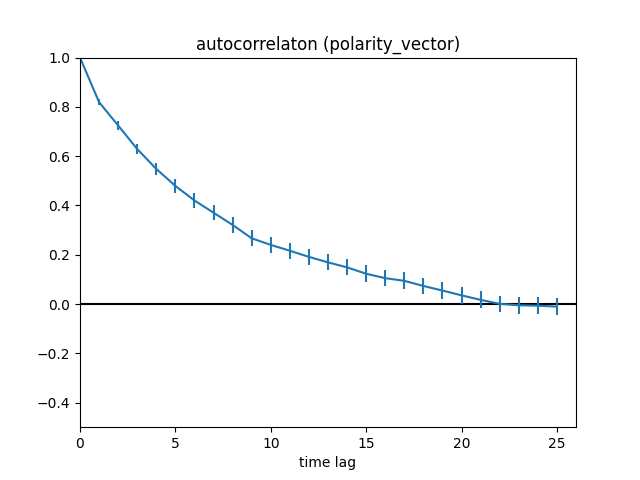
\includegraphics[width=\linewidth]{figures/acf_figures/glass_polarity_vector_acf_avg.png}
      \caption{Autocorrelation for polarity vector on glass}
    \end{subfigure}
    \begin{subfigure}[b]{0.4\linewidth}
      \includegraphics[width=\linewidth]{figures/acf_figures/stiff_polarity_vector_acf_avg.png}
      \caption{Autocorrelation for polarity vector on gel}
    \end{subfigure}
    \caption{The polarity vector has a longer decay on glass than on gel.}
  \end{figure}

\begin{figure}[h!]
    \centering
    \begin{subfigure}[b]{0.4\linewidth}
      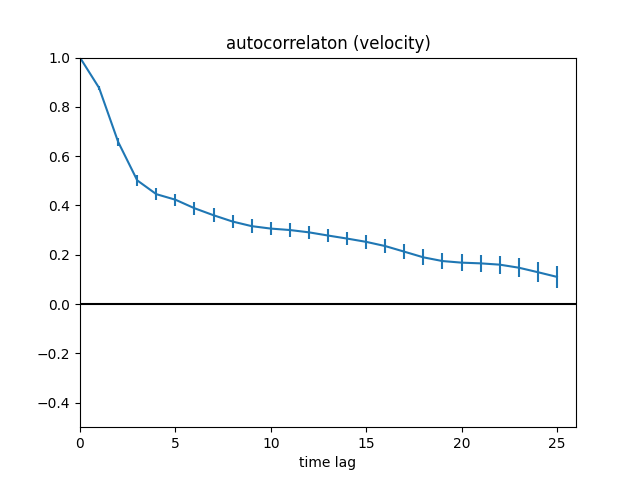
\includegraphics[width=\linewidth]{figures/acf_figures/glass_velocity_acf_avg.png}
      \caption{Autocorrelation for velocity on glass}
    \end{subfigure}
    \begin{subfigure}[b]{0.4\linewidth}
      \includegraphics[width=\linewidth]{figures/acf_figures/stiff_velocity_acf_avg.png}
      \caption{Autocorrelation for velocity on gel}
    \end{subfigure}
    \caption{The velocity has a longer decay on glass than on gel.}
  \end{figure}

\section{Model}
The mathematical model I propose to explain the data is one with two time scale processes, that of the cell polarization and that of the cell
movement direction. I term this model the PRW polarity bias model, or PRWPB. In this model, a number of cells is specified and the length of the simulation is specified, as well as the time step size.
Each cell is initialized with an initial angle for the polarity bias ($\omega_{0}$) and cell direction ($\theta_{0}$) as well as velocity, $v \sim \text{Exp}(3)$. At each time step, the polarity bias
angle is updated as $\omega = \omega_{\text{prev}} + \text{N}(0,\sigma^{2}_{\omega})$ and the cell direction is updated as $\theta = \theta_{\text{prev}} + \text{N}(\omega,\sigma^{2}_{\theta})$.
Cell positions are then determined with $x = x_{\text{prev}} + v \cos(\theta)$ and $y = y_{\text{prev}} + v \sin(\theta)$. I hypothesize that $\sigma_{\omega}^{2} < \sigma_{\theta}^{2}$ in order to 
display the long decay time we observe with the autocorrelations. 

\section{Model Fitting}
For the PRWPB model, there are two parameters to fit: $\sigma^{2}_{\omega}$ and $\sigma^{2}_{\theta}$. To search for the parameters, I perform a grid search. To determine the goodness of the fit, I evaluate
the model fit to the data by either evaluating the fit to the cell average velocity autocorrelation function or to the cell average mean squared displacement (MSD), which is typically how 
models of cell migration are fitted. 

Evaluating the cell averaged fit to the velocity autocorrelation function, we can see that the PRWPB model performs the best (particularly on glass) (Fig. 5) when looking at the velocity autocorrelation (unsurprisingly).

\begin{figure}[h!]
  \centering
  \begin{subfigure}[b]{0.4\linewidth}
    \includegraphics[width=\linewidth]{figures/velacf_model/acf_velocity_modelcomaparion_glass.png }
    \caption{Autocorrelation for velocity on glass}
  \end{subfigure}
  \begin{subfigure}[b]{0.4\linewidth}
    \includegraphics[width=\linewidth]{figures/velacf_model/acf_velocity_modelcomaparion_stiff.png }
    \caption{Autocorrelation for velocity on gel}
  \end{subfigure}
  \caption{Performance of the velocity autocorrelation function with the models, PRWPB and PRW, fitting to the velocity autocorrelation function.}
\end{figure}

And with $D/T$, the PRWPB once again performs the best (Fig. 6).

\begin{figure}[h!]
  \centering
  \begin{subfigure}[b]{0.4\linewidth}
    \includegraphics[width=\linewidth]{figures/velacf_model/DoverT_boxplot_glass.png}
    \caption{$D/T$ on glass}
  \end{subfigure}
  \begin{subfigure}[b]{0.4\linewidth}
    \includegraphics[width=\linewidth]{figures/velacf_model/DoverT_boxplot_stiff.png}
    \caption{$D/T$ on gel}
  \end{subfigure}
  \caption{Performance of $D/T$ with the models, PRWPB and PRW, fitting to the velocity autocorrelation function.}
\end{figure}

However, comparing the MSD, we can see that neither model performs too well in this aspect (Fig. 7).

\begin{figure}[h!]
  \centering
  \begin{subfigure}[b]{0.4\linewidth}
    \includegraphics[width=\linewidth]{figures/velacf_model/MSD_glass.png}
    \caption{MSD on glass}
  \end{subfigure}
  \begin{subfigure}[b]{0.4\linewidth}
    \includegraphics[width=\linewidth]{figures/velacf_model/MSD_stiff.png}
    \caption{MSD on gel}
  \end{subfigure}
  \caption{Performance of the MSD with the models, PRWPB and PRW, fitting to the velocity autocorrelation function.}
\end{figure}

Now, comparing the cell averaged fits to the MSD, looking at the velocity autocorrelation function we can see that once again the PRWPB model does better than the PRW model for glass, but not necessarily gel (Fig. 8).

\begin{figure}[h!]
  \centering
  \begin{subfigure}[b]{0.4\linewidth}
    \includegraphics[width=\linewidth]{figures/MSD_model/acf_velocity_modelcomaparion_glass.png}
    \caption{Autocorrelation for velocity on glass}
  \end{subfigure}
  \begin{subfigure}[b]{0.4\linewidth}
    \includegraphics[width=\linewidth]{figures/MSD_model/acf_velocity_modelcomaparion_stiff.png}
    \caption{Autocorrelation for velocity on gel}
  \end{subfigure}
  \caption{Performance of the velocity autocorrelation function with the models, PRWPB and PRW, fitting to the MSD.}
\end{figure}

And looking at the comparisons for $D/T$, the PRWPB does better for glass but not for gel (Fig. 9)

\begin{figure}[h!]
  \centering
  \begin{subfigure}[b]{0.4\linewidth}
    \includegraphics[width=\linewidth]{figures/MSD_model/DoverT_boxplot_glass.png}
    \caption{$D/T$ on glass}
  \end{subfigure}
  \begin{subfigure}[b]{0.4\linewidth}
    \includegraphics[width=\linewidth]{figures/MSD_model/DoverT_boxplot_stiff.png}
    \caption{$D/T$ on gel}
  \end{subfigure}
  \caption{Performance of $D/T$ with the models, PRWPB and PRW, fitting to the MSD.}
\end{figure}

And looking at the MSD the PRWPB does not represent the MSD well on gel or glass (Fig. 10).

\begin{figure}[h!]
  \centering
  \begin{subfigure}[b]{0.4\linewidth}
    \includegraphics[width=\linewidth]{figures/MSD_model/MSD_glass.png}
    \caption{MSD on glass}
  \end{subfigure}
  \begin{subfigure}[b]{0.4\linewidth}
    \includegraphics[width=\linewidth]{figures/MSD_model/MSD_stiff.png}
    \caption{MSD on gel}
  \end{subfigure}
  \caption{Performance of the MSD with the models, PRWPB and PRW, fitting to the MSD.}
\end{figure}

I also tried fitting to each cell individually, which I call the heterogeneous fit, to both the velocity autocorrelation function and the MSD.

Evaluating the velocity autocorrelation for the heterogeneous velocity autocorrelation fits, we can see that the PRWPB model performs well for both glass and gel, but 
not quite as good as the cell averaged velocity autocorrelation fit (Fig. 11). 

\begin{figure}[h!]
  \centering
  \begin{subfigure}[b]{0.4\linewidth}
    \includegraphics[width=\linewidth]{figures/velacf_hetero_model/acf_velocity_modelcomaparion_glass.png}
    \caption{Autocorrelation for velocity on glass}
  \end{subfigure}
  \begin{subfigure}[b]{0.4\linewidth}
    \includegraphics[width=\linewidth]{figures/velacf_hetero_model/acf_velocity_modelcomaparion_stiff.png}
    \caption{Autocorrelation for velocity on gel}
  \end{subfigure}
  \caption{Performance of the velocity autocorrelation function with the models, PRWPB and PRW, fitting to the heterogeneous velocity autocorrelation function.}
\end{figure}

The $D/T$ is captured best by the PRWPB on stiff but not as well on glass with the heterogeneous velocity autocorrelation fit (Fig. 12)

\begin{figure}[h!]
  \centering
  \begin{subfigure}[b]{0.4\linewidth}
    \includegraphics[width=\linewidth]{figures/MSD_model/DoverT_boxplot_glass.png}
    \caption{$D/T$ on glass}
  \end{subfigure}
  \begin{subfigure}[b]{0.4\linewidth}
    \includegraphics[width=\linewidth]{figures/MSD_model/DoverT_boxplot_stiff.png}
    \caption{$D/T$ on gel}
  \end{subfigure}
  \caption{Performance of $D/T$ with the models, PRWPB and PRW, fitting to the heterogeneous velocity autocorrelation function.}
\end{figure}

Looking at the MSD for this fit, the PRWPB does better than the PRW (Fig. 13).

\begin{figure}[h!]
  \centering
  \begin{subfigure}[b]{0.4\linewidth}
    \includegraphics[width=\linewidth]{figures/velacf_hetero_model/MSD_glass.png}
    \caption{MSD on glass}
  \end{subfigure}
  \begin{subfigure}[b]{0.4\linewidth}
    \includegraphics[width=\linewidth]{figures/velacf_hetero_model/MSD_stiff.png}
    \caption{MSD on gel}
  \end{subfigure}
  \caption{Performance of the MSD with the models, PRWPB and PRW, fitting to the heterogeneous velocity autocorrelation function.}
\end{figure}

Now, evaluating the heterogeneous MSD fits, we can see that the velocity autocorrelation function shows that the PRWPB shows a better fit (Fig. 14).

\begin{figure}[h!]
  \centering
  \begin{subfigure}[b]{0.4\linewidth}
    \includegraphics[width=\linewidth]{figures/MSD_hetero_model/acf_velocity_modelcomaparion_glass.png}
    \caption{Autocorrelation for velocity on glass}
  \end{subfigure}
  \begin{subfigure}[b]{0.4\linewidth}
    \includegraphics[width=\linewidth]{figures/MSD_hetero_model/acf_velocity_modelcomaparion_stiff.png}
    \caption{Autocorrelation for velocity on gel}
  \end{subfigure}
  \caption{Performance of the velocity autocorrelation function with the models, PRWPB and PRW, fitting to the heterogeneous MSD.}
\end{figure}

And looking at $D/T$ for the heterogeneous MSD fits, the PRWPB model performs better on both glass and gel (Fig. 15).

\begin{figure}[h!]
  \centering
  \begin{subfigure}[b]{0.4\linewidth}
    \includegraphics[width=\linewidth]{figures/MSD_hetero_model/DoverT_boxplot_glass.png}
    \caption{$D/T$ on glass}
  \end{subfigure}
  \begin{subfigure}[b]{0.4\linewidth}
    \includegraphics[width=\linewidth]{figures/MSD_hetero_model/DoverT_boxplot_stiff.png}
    \caption{$D/T$ on gel}
  \end{subfigure}
  \caption{Performance of $D/T$ with the models, PRWPB and PRW, fitting to the heterogeneous MSD.}
\end{figure}

And evaluating the MSD, once again the PRWPB does a little better here too (Fig. 12).

\begin{figure}[h!]
  \centering
  \begin{subfigure}[b]{0.4\linewidth}
    \includegraphics[width=\linewidth]{figures/MSD_hetero_model/MSD_glass.png}
    \caption{MSD on glass}
  \end{subfigure}
  \begin{subfigure}[b]{0.4\linewidth}
    \includegraphics[width=\linewidth]{figures/MSD_hetero_model/MSD_stiff.png}
    \caption{MSD on gel}
  \end{subfigure}
  \caption{Performance of the MSD with the models, PRWPB and PRW, fitting to the heterogeneous MSD.}
\end{figure}

\section{Conclusions and Future Directions}

From this analysis, we have found that step size in $x$ and $y$ is not statistically different on glass and gel, however $D/T$ and speed are.
Furthermore, cells migrating on glass and gel display different decay times in the autocorrelatoin function with both velocity and polarity.
I have created a model that out-performs the traditional PRW model used to model cell migration in almost every case (glass vs gel, MSD vs velocity autocorrelation fit,
cell averaged vs heterogeneous fit), but more often on glass than gel since glass is where we observe the most deviation from the PRW with the prolonged autocorrelation decay times.
Since glass is stiffer than gel, it appears that the stiffer the substrate, the slower a cell moves with less change in velocity over time.

However, there is still much to be evaluated. Firstly, shape needs to be incorporated into the model. Additionally, more shape metrics need to be evalued on glass vs gel rather
than just the autocorrelation of the polarity vector. Not only that, but more exploratory analyses could be performed on this data. For instance, could we use k-means clustering
to gain insight in the motion and shape metrics on each substrate? It would be interesting to see if we could cluster based on substrate for these metrics if time permitted. 

\begin{thebibliography}{4}

  \bibitem{Malik} Malik AA, Gerlee P. Mathematical modelling of cell migration: stiffness dependent jump rates result in durotaxis. 
   \emph{J Math Biol}. 2019;78(7):2289-2315. doi:10.1007/s00285-019-01344-5

  \bibitem{Shellard} Shellard A, Mayor R. Durotaxis: The Hard Path from In Vitro to In Vivo. 
   \emph{Dev Cell}. 2021;56(2):227-239. doi:10.1016/j.devcel.2020.11.019

  \bibitem{Stefanoni} Stefanoni F, Ventre M, Mollica F, Netti PA. A numerical model for durotaxis. 
   \emph{J Theor Biol}. 2011;280(1):150-158. doi:10.1016/j.jtbi.2011.04.001

  \bibitem{Wu} Wu PH, Giri A, Sun SX, Wirtz D. Three-dimensional cell migration does not follow a random walk. 
   \emph{Proc Natl Acad Sci USA}. 2014;111(11):3949-3954. doi:10.1073/pnas.1318967111

\end{thebibliography}

\end{document}
